\section{Task 1}

\subsection{Distribution of Machine Check Exceptions}

In order to compare this distribution of machine check exceptions across all node types, we first must define what we consider ``memory'', ``L1'' and ``L2'' errors.  For the purposes of this (and future) problems, we define:

\begin{verbatim}
L1_errors <- c("L1 cache Fill ECC error", "L1 tag load", "L1 TLB IC load")
L2_errors <- c("L2 cache Fill ECC error", "L2 cache Fill ECC Error", "L2 ECC Error", "L2 IC cache parity error", "L2 TLB")
mem_errors <- c("DRAM Parity Error", "ECC Error")
\end{verbatim}

We do not include \fix{"NB Array Error"} in any of these categories, as the AMD manual explicitly distinguishes between the northbridge and memory.  The \fix{"Table Walk Data Error"}, \fix{"Data copy back Evict"}, and \fix{"Link Retry"} errors do not directly involve the main memory, L1, or L2 caches.

Once we defined these categories, we filtered the data by both type and node type and used \fix{nrow} to determine the number (and, by dividing, percentage) of entries in each category.

The results of this distribution exercise are shown below:

\begin{table}[ht]
\centering
\begin{tabular}{rllrr}
  \hline
 & nodeType & type & nerr & perr \\ 
  \hline
1 & compute & L1 & 210 & 0.02 \\ 
  2 & compute & L2 & 177 & 0.01 \\ 
  3 & compute & mem & 8848 & 0.74 \\ 
  4 & compute & other & 2685 & 0.23 \\ 
  5 & GPU & L1 &   2 & 0.00 \\ 
  6 & GPU & L2 &  14 & 0.02 \\ 
  7 & GPU & mem & 616 & 0.91 \\ 
  8 & GPU & other &  48 & 0.07 \\ 
  9 & lnet & L1 &   0 & 0.00 \\ 
  10 & lnet & L2 &   0 & 0.00 \\ 
  11 & lnet & mem &   7 & 0.64 \\ 
  12 & lnet & other &   4 & 0.36 \\ 
  13 & service & L1 &   4 & 0.00 \\ 
  14 & service & L2 &  38 & 0.01 \\ 
  15 & service & mem & 2382 & 0.62 \\ 
  16 & service & other & 1411 & 0.37 \\ 
  17 & mom & L1 &   0 & 0.00 \\ 
  18 & mom & L2 &   0 & 0.00 \\ 
  19 & mom & mem &  76 & 0.97 \\ 
  20 & mom & other &   2 & 0.03 \\ 
  21 & all & L1 & 216 & 0.01 \\ 
  22 & all & L2 & 229 & 0.01 \\ 
  23 & all & mem & 11929 & 0.72 \\ 
  24 & all & other & 4150 & 0.25 \\ 
   \hline
\end{tabular}
\end{table}

Generally speaking, memory errors account for the majority of errors encountered in the data, while L1 and L2 cache errors are relatively rare.

To compute the MTBFs across banks and these extended types, we used the same formula discussed in Task 0 to calculate the MTBF across the subsetted data set.

The results of this experiment are shown below:

\begin{table}[t]
\centering
\begin{tabular}{rrllr}
  \hline
 & bank & nodeType & type & mtbf \\ 
  \hline
1 &   4 & compute & L1 & Inf \\ 
  2 &   4 & compute & L2 & Inf \\ 
  3 &   4 & compute & mem & 0.02 \\ 
  4 &   4 & compute & other & 0.07 \\ 
  5 &   4 & GPU & L1 & Inf \\ 
  6 &   4 & GPU & L2 & Inf \\ 
  7 &   4 & GPU & mem & 0.31 \\ 
  8 &   4 & GPU & other & 4.00 \\ 
  9 &   4 & lnet & L1 & Inf \\ 
  10 &   4 & lnet & L2 & Inf \\ 
  11 &   4 & lnet & mem & 27.43 \\ 
  12 &   4 & lnet & other & 48.00 \\ 
  13 &   4 & service & L1 & Inf \\ 
  14 &   4 & service & L2 & Inf \\ 
  15 &   4 & service & mem & 0.08 \\ 
  16 &   4 & service & other & 0.14 \\ 
  17 &   4 & mom & L1 & Inf \\ 
  18 &   4 & mom & L2 & Inf \\ 
  19 &   4 & mom & mem & 2.53 \\ 
  20 &   4 & mom & other & 96.00 \\ 
  21 &   4 & all & L1 & Inf \\ 
  22 &   4 & all & L2 & Inf \\ 
  23 &   4 & all & mem & 0.02 \\ 
  24 &   4 & all & other & 0.05 \\

   \hline
\end{tabular}
\end{table}

\begin{t able}[t]
\centering
\begin{tabular}{rrllr}
  \hline
 & bank & nodeType & type & mtbf \\ 
  \hline
  25 &   1 & compute & L1 & 0.96 \\ 
  26 &   1 & compute & L2 & 14.77 \\ 
  27 &   1 & compute & mem & Inf \\ 
  28 &   1 & compute & other & Inf \\ 
  29 &   1 & GPU & L1 & 192.00 \\ 
  30 &   1 & GPU & L2 & Inf \\ 
  31 &   1 & GPU & mem & Inf \\ 
  32 &   1 & GPU & other & Inf \\ 
  33 &   1 & lnet & L1 & Inf \\ 
  34 &   1 & lnet & L2 & Inf \\ 
  35 &   1 & lnet & mem & Inf \\ 
  36 &   1 & lnet & other & Inf \\ 
  37 &   1 & service & L1 & 96.00 \\ 
  38 &   1 & service & L2 & Inf \\ 
  39 &   1 & service & mem & Inf \\ 
  40 &   1 & service & other & Inf \\ 
  41 &   1 & mom & L1 & Inf \\ 
  42 &   1 & mom & L2 & Inf \\ 
  43 &   1 & mom & mem & Inf \\ 
  44 &   1 & mom & other & Inf \\ 
  45 &   1 & all & L1 & 0.95 \\ 
  46 &   1 & all & L2 & 14.77 \\ 
  47 &   1 & all & mem & Inf \\ 
  48 &   1 & all & other & Inf \\ 
 
   \hline
\end{tabular}
\end{table}

\begin{table}[t]
\centering
\begin{tabular}{rrllr}
  \hline
 & bank & nodeType & type & mtbf \\ 
  \hline
  49 &   2 & compute & L1 & 32.00 \\ 
  50 &   2 & compute & L2 & 1.17 \\ 
  51 &   2 & compute & mem & Inf \\ 
  52 &   2 & compute & other & 192.00 \\ 
  53 &   2 & GPU & L1 & Inf \\ 
  54 &   2 & GPU & L2 & 13.71 \\ 
  55 &   2 & GPU & mem & Inf \\ 
  56 &   2 & GPU & other & Inf \\ 
  57 &   2 & lnet & L1 & Inf \\ 
  58 &   2 & lnet & L2 & Inf \\ 
  59 &   2 & lnet & mem & Inf \\ 
  60 &   2 & lnet & other & Inf \\ 
  61 &   2 & service & L1 & 96.00 \\ 
  62 &   2 & service & L2 & 5.05 \\ 
  63 &   2 & service & mem & Inf \\ 
  64 &   2 & service & other & Inf \\ 
  65 &   2 & mom & L1 & Inf \\ 
  66 &   2 & mom & L2 & Inf \\ 
  67 &   2 & mom & mem & Inf \\ 
  68 &   2 & mom & other & Inf \\ 
  69 &   2 & all & L1 & 24.00 \\ 
  70 &   2 & all & L2 & 0.89 \\ 
  71 &   2 & all & mem & Inf \\ 
  72 &   2 & all & other & 192.00 \\

   \hline
\end{tabular}
\end{table}

\begin{table}[t]
\centering
\begin{tabular}{rrllr}
  \hline
 & bank & nodeType & type & mtbf \\ 
  \hline
  73 &   0 & compute & L1 & 48.00 \\ 
  74 &   0 & compute & L2 & Inf \\ 
  75 &   0 & compute & mem & Inf \\ 
  76 &   0 & compute & other & Inf \\ 
  77 &   0 & GPU & L1 & 192.00 \\ 
  78 &   0 & GPU & L2 & Inf \\ 
  79 &   0 & GPU & mem & Inf \\ 
  80 &   0 & GPU & other & Inf \\ 
  81 &   0 & lnet & L1 & Inf \\ 
  82 &   0 & lnet & L2 & Inf \\ 
  83 &   0 & lnet & mem & Inf \\ 
  84 &   0 & lnet & other & Inf \\ 
  85 &   0 & service & L1 & Inf \\ 
  86 &   0 & service & L2 & Inf \\ 
  87 &   0 & service & mem & Inf \\ 
  88 &   0 & service & other & Inf \\ 
  89 &   0 & mom & L1 & Inf \\ 
  90 &   0 & mom & L2 & Inf \\ 
  91 &   0 & mom & mem & Inf \\ 
  92 &   0 & mom & other & Inf \\ 
  93 &   0 & all & L1 & 38.40 \\ 
  94 &   0 & all & L2 & Inf \\ 
  95 &   0 & all & mem & Inf \\ 
  96 &   0 & all & other & Inf \\ 
   \hline
\end{tabular}
\end{table}


Note that the MTBFs across different node types are very different: the MTBF for bank 4 memory errors varies from about 0.02 hours (\fix{compute}) to about 27 hours (\fix{lnet}).  There are a few possibilities for the cause of these results:

\begin{itemize}
\item Different types of nodes have different quantities of memory and cache; if more memory is present, MTBFs should be lower as there are more components that can fail.
\item Different types of nodes have different utilization percentages: it is possible that the routing nodes (\fix{lnet, mom}) are used less relative to their maximum capacity versus compute nodes (for example), leading to smaller MTBFs.
\end{itemize}

There are two uncorrectable errors in our data set, yielding an MTBF of 96 hours and a FIT of approximately $1.042 \cdot 10^7$.  One error occured in bank 0 of a compute node and was an L1 error, while the second error occured in bank 4 of a compute node and was a memory error.  If we wish to separate the uncorrectable errors by bank, node type, or type, the two resulting entries would individually have MTBF values of 192 hours and FIT values of $5.208 \cdot 10^6$.

\subsection{Time Between Consecutive Failures}
\subsubsection{Plotting the Daily MTBF}

In order to compute the MTBF per day, we can subset the data by days.  The easiest way to do this is to convert ``October 6, 2012 12:00 AM CDT'' into a Unix timestamp and use the fact that there are 86,400 seconds in a day to create upper and lower bounds for a given day's timestamp.  Once we have filtered this data, we can calculate MTBF by dividing 86400 seconds by the number of failures in the filtered data.  By concatenating the results for every day together, we can plot this data on a graph.

The graphs for each day are shown below:

\begin{figure}
\centering
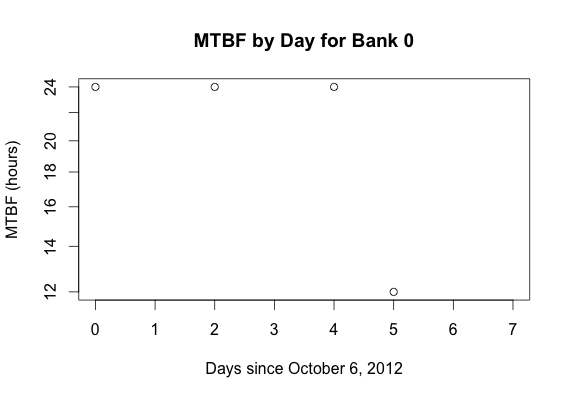
\includegraphics[width=0.45\textwidth]{images/mtbf_0.png}
\end{figure}

\begin{figure}
\centering
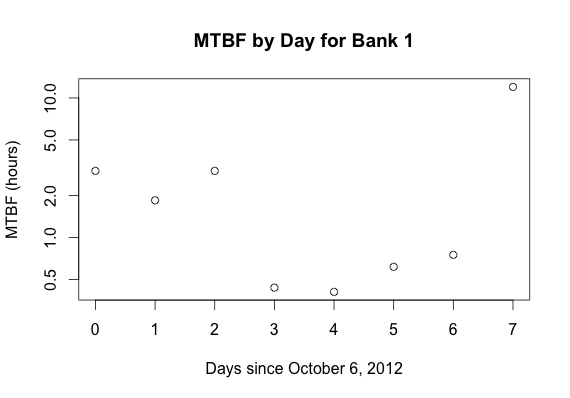
\includegraphics[width=0.45\textwidth]{images/mtbf_1.png}
\end{figure}

\begin{figure}
\centering
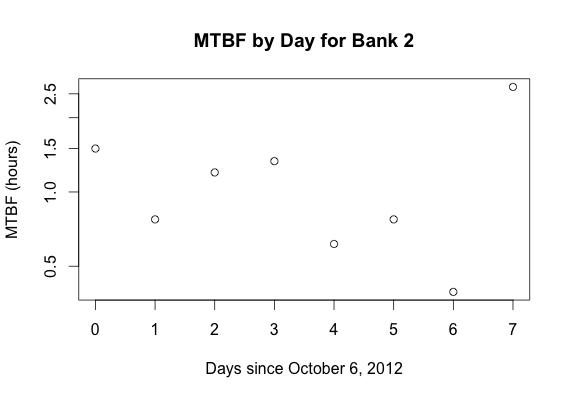
\includegraphics[width=0.45\textwidth]{images/mtbf_2.png}
\end{figure}

\begin{figure}
\centering
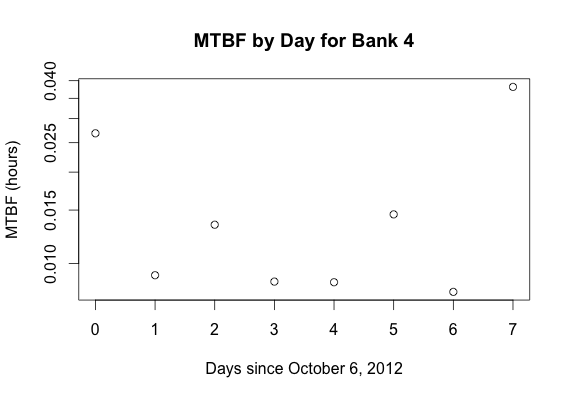
\includegraphics[width=0.45\textwidth]{images/mtbf_4.png}
\end{figure}

\subsubsection{Plotting the TBFs}

The \fix{diff} command can be used on a vector of numeric values to return the differences between subsequent values.  If we call \fix{diff} on a set of filtered data, we can use the \fix{hist} command to visualize the time between failures.

The plots for the TBFs are shown below.  Note that we do not create a histogram for categories that only have one point of data in them (as it is impossible to create a sensible time between failure amount there)--as a result, the graph for all node types may differ significantly from the individual graph categories due to the addition of these one-item categories.


\begin{figure}
\centering
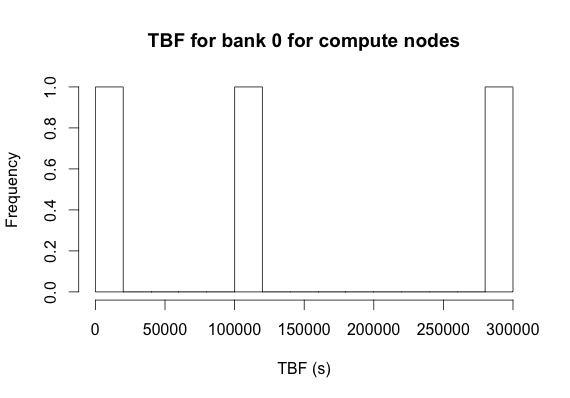
\includegraphics[width=0.45\textwidth]{images/tbf_0_c.png}
\end{figure}

\begin{figure}
\centering
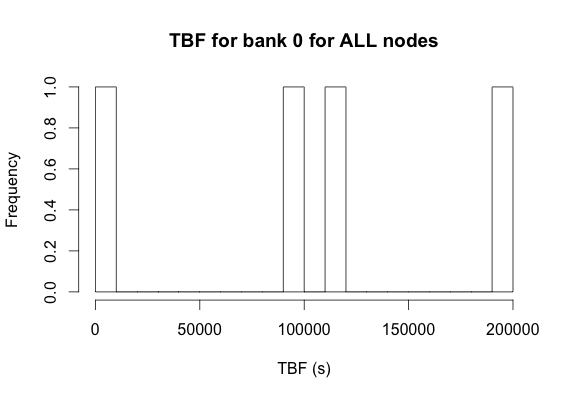
\includegraphics[width=0.45\textwidth]{images/tbf_0_a.png}
\end{figure}

\begin{figure}
\centering
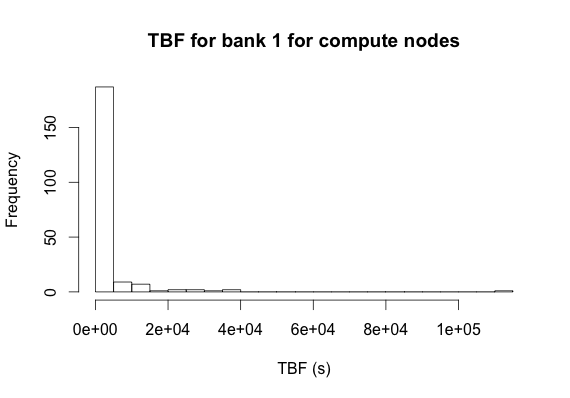
\includegraphics[width=0.45\textwidth]{images/tbf_1_c.png}
\end{figure}

\begin{figure}
\centering
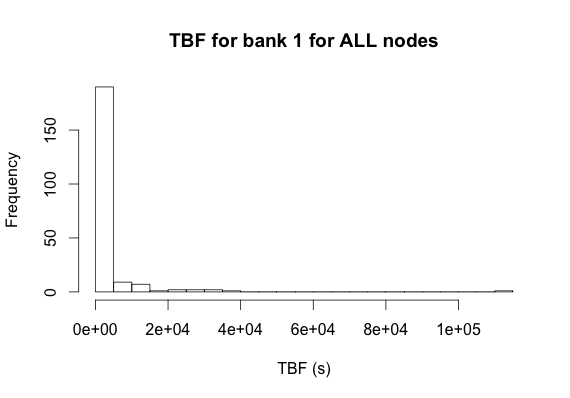
\includegraphics[width=0.45\textwidth]{images/tbf_1_a.png}
\end{figure}

\begin{figure}
\centering
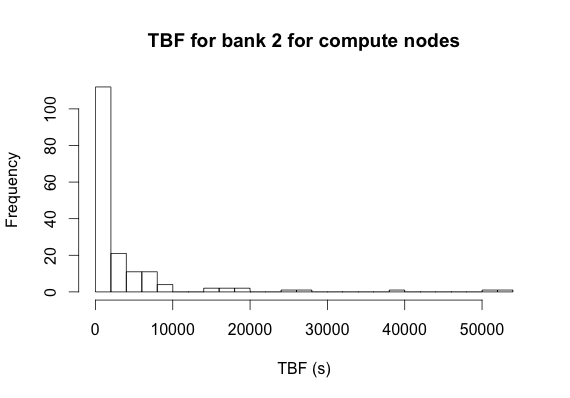
\includegraphics[width=0.45\textwidth]{images/tbf_2_c.png}
\end{figure}

\begin{figure}
\centering
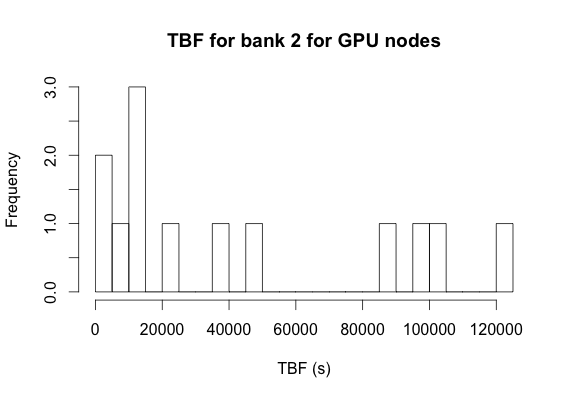
\includegraphics[width=0.45\textwidth]{images/tbf_2_g.png}
\end{figure}

\begin{figure}
\centering
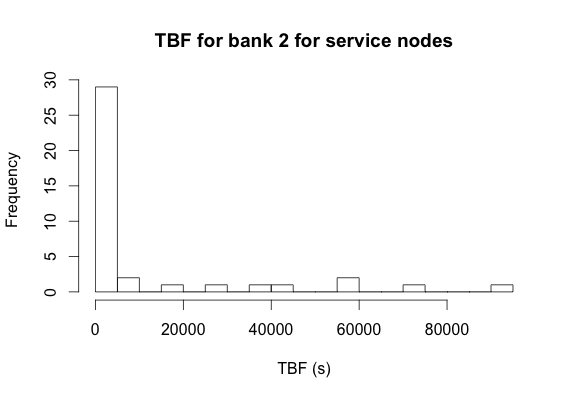
\includegraphics[width=0.45\textwidth]{images/tbf_2_s.png}
\end{figure}

\begin{figure}
\centering
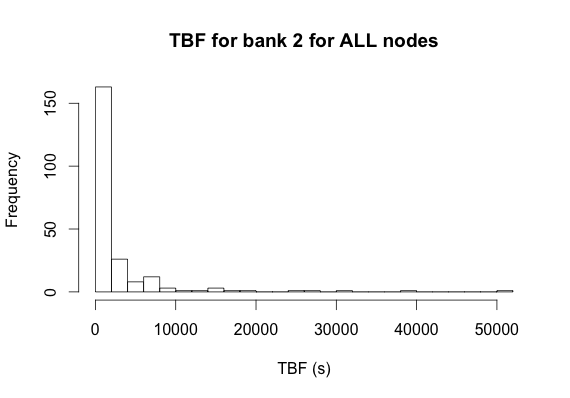
\includegraphics[width=0.45\textwidth]{images/tbf_2_a.png}
\end{figure}

\begin{figure}
\centering
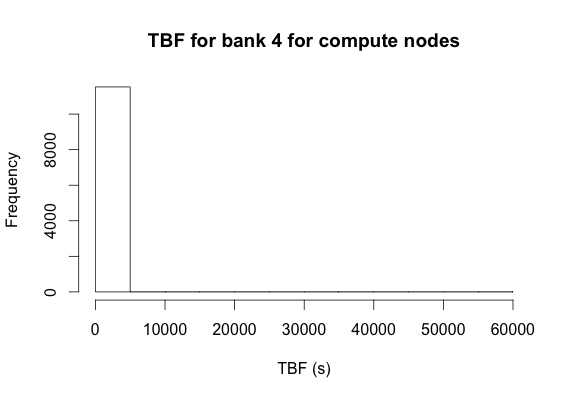
\includegraphics[width=0.45\textwidth]{images/tbf_4_c.png}
\end{figure}

\begin{figure}
\centering
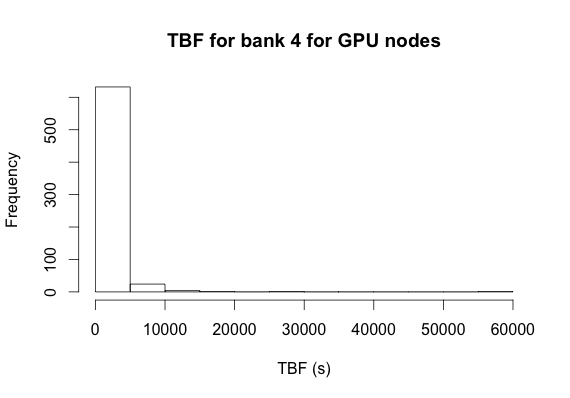
\includegraphics[width=0.45\textwidth]{images/tbf_4_g.png}
\end{figure}

\begin{figure}
\centering
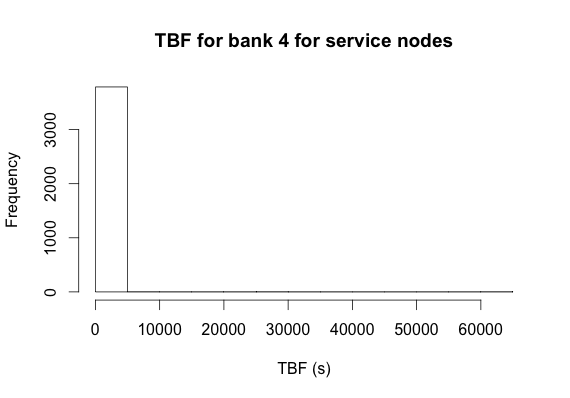
\includegraphics[width=0.45\textwidth]{images/tbf_4_s.png}
\end{figure}

\begin{figure}
\centering
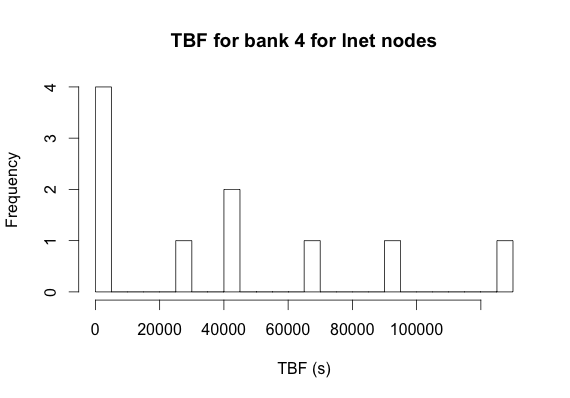
\includegraphics[width=0.45\textwidth]{images/tbf_4_l.png}
\end{figure}

\begin{figure}
\centering
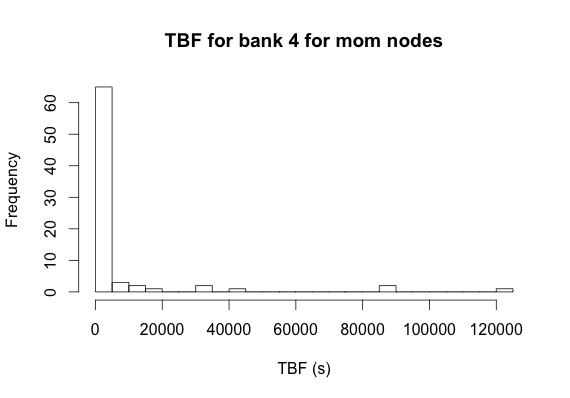
\includegraphics[width=0.45\textwidth]{images/tbf_4_m.png}
\end{figure}

\begin{figure}
\centering
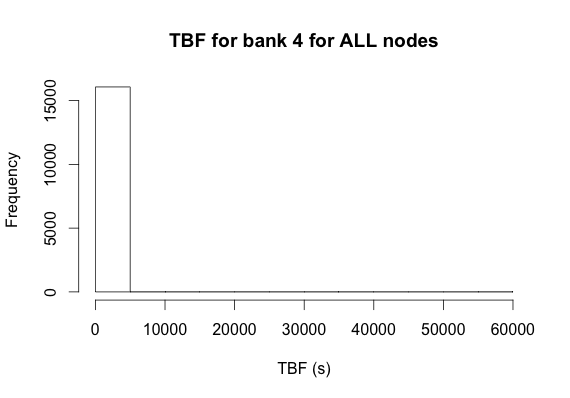
\includegraphics[width=0.45\textwidth]{images/tbf_4_a.png}
\end{figure}

\subsubsection{Plotting the Hazard Rate}

First, note that our hazard rate analysis is necessarily limited by our data set--ideally, we would able to track failures over the entire lifetime of the hardware.  Given these circumstances, we decided to shift our timestamp data to define our origin time as the start of October 6 (12:00 AM CDT) and run \fix{muhaz} on this data.  Note that \code{muhaz} defines its \code{max.time} field based on when ``ten patients remain at risk''\cite{MUHAZ}.  As such, we did not plot the hazard rates for categories that contained fewer than 11 separate timestamps (10 diffs).

The hazard rate plots are shown below:

\begin{figure}
\centering
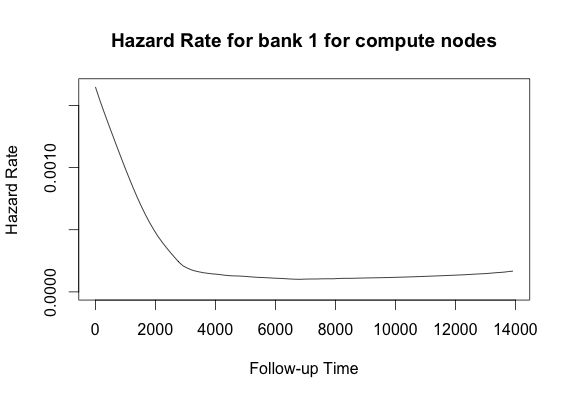
\includegraphics[width=0.45\textwidth]{images/haz_1_c.png}
\end{figure}

\begin{figure}
\centering
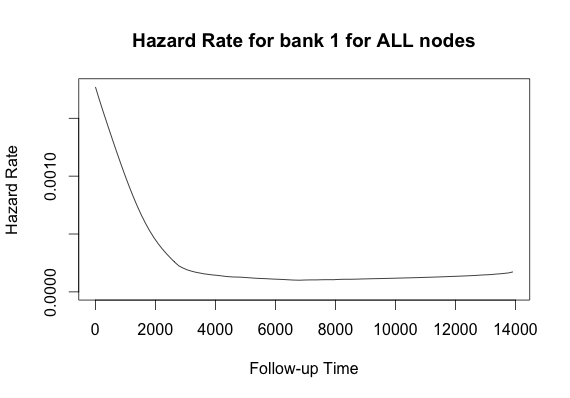
\includegraphics[width=0.45\textwidth]{images/haz_1_a.png}
\end{figure}

\begin{figure}
\centering
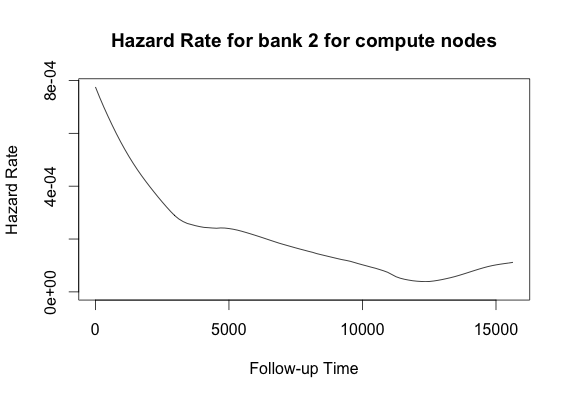
\includegraphics[width=0.45\textwidth]{images/haz_2_c.png}
\end{figure}

\begin{figure}
\centering
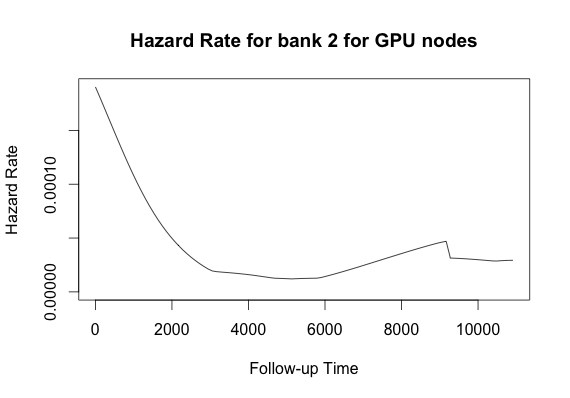
\includegraphics[width=0.45\textwidth]{images/haz_2_g.png}
\end{figure}

\begin{figure}
\centering
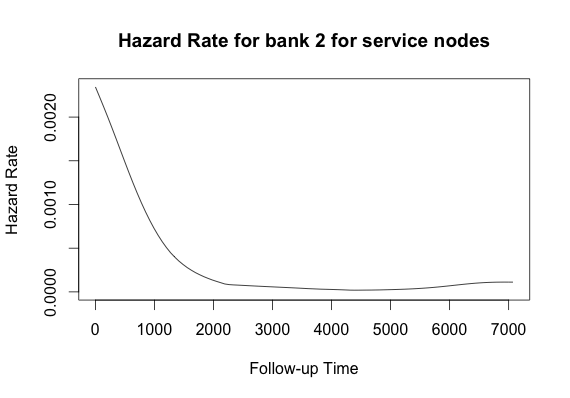
\includegraphics[width=0.45\textwidth]{images/haz_2_s.png}
\end{figure}

\begin{figure}
\centering
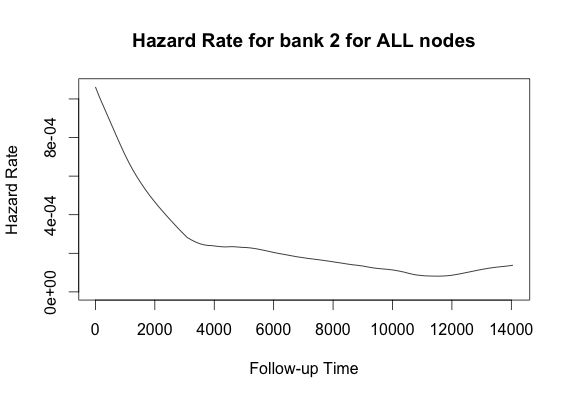
\includegraphics[width=0.45\textwidth]{images/haz_2_a.png}
\end{figure}

\begin{figure}
\centering
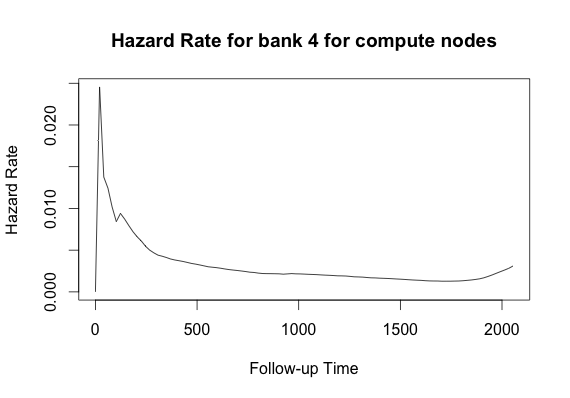
\includegraphics[width=0.45\textwidth]{images/haz_4_c.png}
\end{figure}

\begin{figure}
\centering
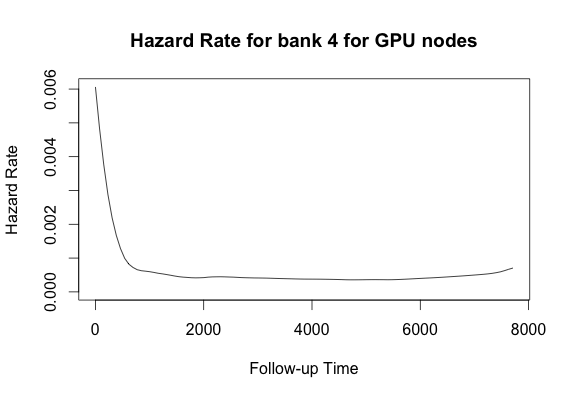
\includegraphics[width=0.45\textwidth]{images/haz_4_g.png}
\end{figure}

\begin{figure}
\centering
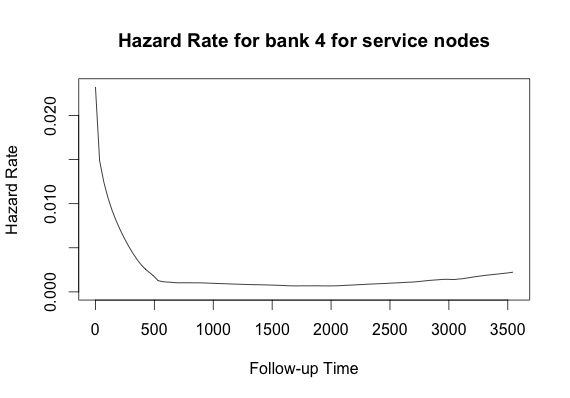
\includegraphics[width=0.45\textwidth]{images/haz_4_s.png}
\end{figure}

\begin{figure}
\centering
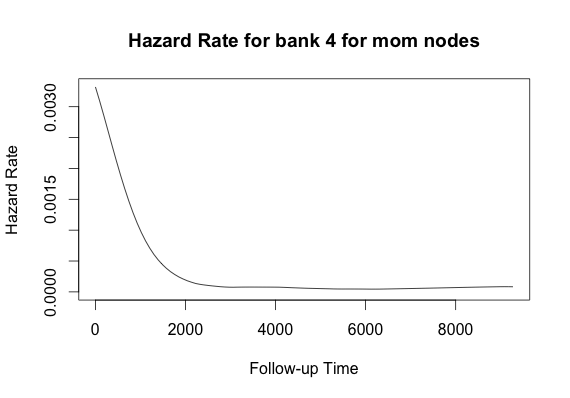
\includegraphics[width=0.45\textwidth]{images/haz_4_m.png}
\end{figure}

\begin{figure}
\centering
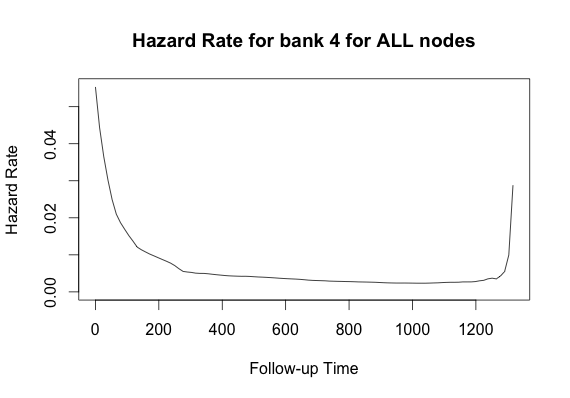
\includegraphics[width=0.45\textwidth]{images/haz_4_a.png}
\end{figure}

\subsubsection{Analysis}

We derived the following insights based on our results:

\begin{itemize}
\item The MTBF for each day does not appear to be comparable across banks for different days.  We believe that this could be the case because of the relatively small size of our data set; as a result, noise due to other factors (system load, for example) dominated any other trends in the data.  One small trend is that Saturdays (days 0 and 7) appeared to have higher MTBFs than other data throughout the week, but we are not sure if this trend is statistically significant.
\item The time between failures appears to trend significantly towards small numbers.  We believe that one reason that this occurs is because failures may occur more often during heavy use; if a failure happens, the machine is more likely to be under more load, so more failures are likely to follow.  Similarly, permanent hardware failures and cosmic ray strikes are likely to be localized to a small area, and processors tend to access physically-close regions of memory over a short period of time; as a result, when a failure occurs, other failures should be likely to occur in a short time.
\item The hazard rate generally decreases (often significantly) as time goes on.  Intuitively, this is the case because times between failure are generally short in this system; if a piece of hardware is going to fail, it is far more likely to do so close to the failure of another piece of hardware (possibly due to the factors mentioned in the previous point).
\end{itemize}
